\documentclass{standalone}
% Preamble
\begin{document}


\subsection{Structure bloc-triangulaire et rang numérique de $B(1)$}
Dans le processus de réduction, la première étape consiste à calculer le noyau de $B(1)$. Lorsque les coefficients des polynômes d'entrée sont entiers ou rationnels, ceci peut se faire de manière exacte au moyen d'un programme de calcul symbolique. La taille des entiers peut alors croître considérablement au cours des calculs et augmenter en conséquence le temps total de calcul et les besoins en mémoire du calculateur. Si par contre on veut effectuer l'ensemble des calculs en nombres flottants, ou si les coefficients d'entrée sont eux mêmes donnés sous forme numérique, alors on doit faire un calcul numérique du noyau.
La méthode éprouvée pour cela, implémentée dans des packages d'algèbre linéaire numérique comme Matlab/Octave, Numpy ou Julia, est d'effectuer une factorisation QR ``rank revealing'' de $B(1)$, que nous appellerons factorisation QRP, c'est-à-dire accompagnée de pivots sur les colonnnes. L'expérience montre que cette approche est souvent efficace mais peut s'avérer délicate à mettre en oeuvre si la taille de la matrice augmente. Montrons le sur un exemple.

\begin{exmp}
Nous choisissons $n = 4$,
\begin{align}
f_1 & = x_0^2x_1^2x_2x_3^2 - x_0^2x_1x_2^2x_3^2 - x_0^3x_1x_3^2 + x_0x_1^2x_2x_3^2 + x_0x_1^2x_3^2 + x_0^3x_2 - x_1^2x_3^2 + x_0^2x_2 + x_0x_1x_2 + x_1x_2x_3 + x_2^2 + x_2x_3 + 1,\nonumber\\
f_2 & = x_0^3x_1^2x_2x_3^2 + x_0^3x_1x_2^2 - x_0^2x_1^2x_2^2 + x_0^2x_1x_2x_3^2 - x_0^3x_1^2 + x_0^2x_1^2x_3 - x_0^3x_2x_3 + x_0x_1x_2^2x_3 + x_0^3x_3^2 - x_0x_1x_2x_3^2 + x_0x_1x_2^2 - x_0^3x_3 + x_0x_1x_2x_3 + x_1^2x_2x_3 - x_1^2x_3^2 - x_0^2x_1 + x_0x_1 + x_2^2 + x_3^2 - x_1 + 1,\nonumber\\
f_3 & =  -x_0^2x_1^2x_2^2x_3^2 - x_0^3x_1^2x_2x_3 - x_0^3x_2^2x_3^2 - x_0^3x_1x_2x_3 + x_0x_1x_2^2x_3^2 + x_0^3x_1 - x_1x_2x_3^2 + x_2^2x_3^2 + x_1^2x_3 - x_0x_2x_3 + x_0^2 + x_2^2 - x_0x_3 + x_1,\nonumber\\
f_4 & =  x_0^2x_1^2x_2^2x_3 + x_0^3x_1x_3^2 - x_0^3x_1x_2 - x_0^3x_3^2 - x_0x_1^2x_3^2 - x_0x_1x_2x_3 - x_1^2x_3^2 + x_1x_2^2 - x_1x_3^2 + x_3^2 - x_0 - 1 \nonumber
\end{align}
\end{exmp}
\begin{center}
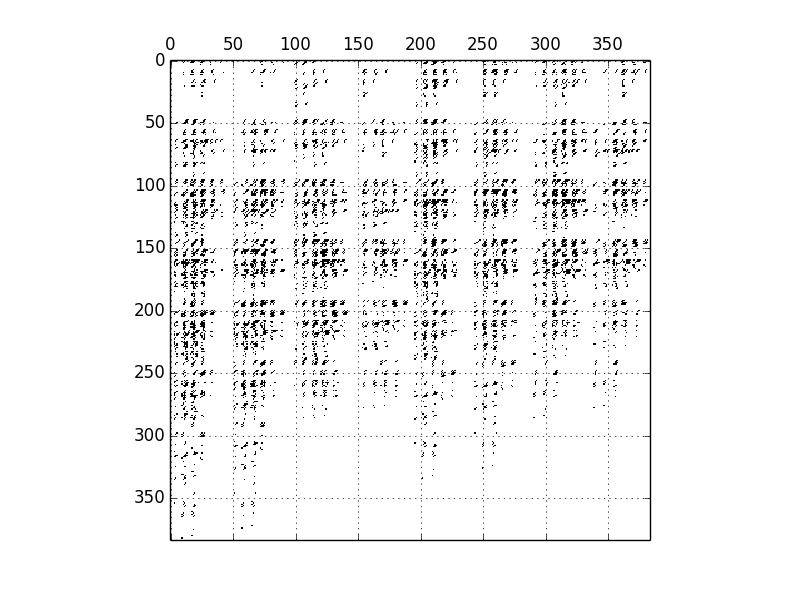
\includegraphics[width=8cm]{B0.png}
\end{center}

Ce système est de multidegré $(3, 2, 2, 2)$, la matrice de Bezout $B(1)$ est de taille $576$. Si on effectue une factorisation QRP sur cette matrice, on sait que les éléments diagonaux seront triés en ordre décroissant, voir figure ci-dessous.
\begin{center}
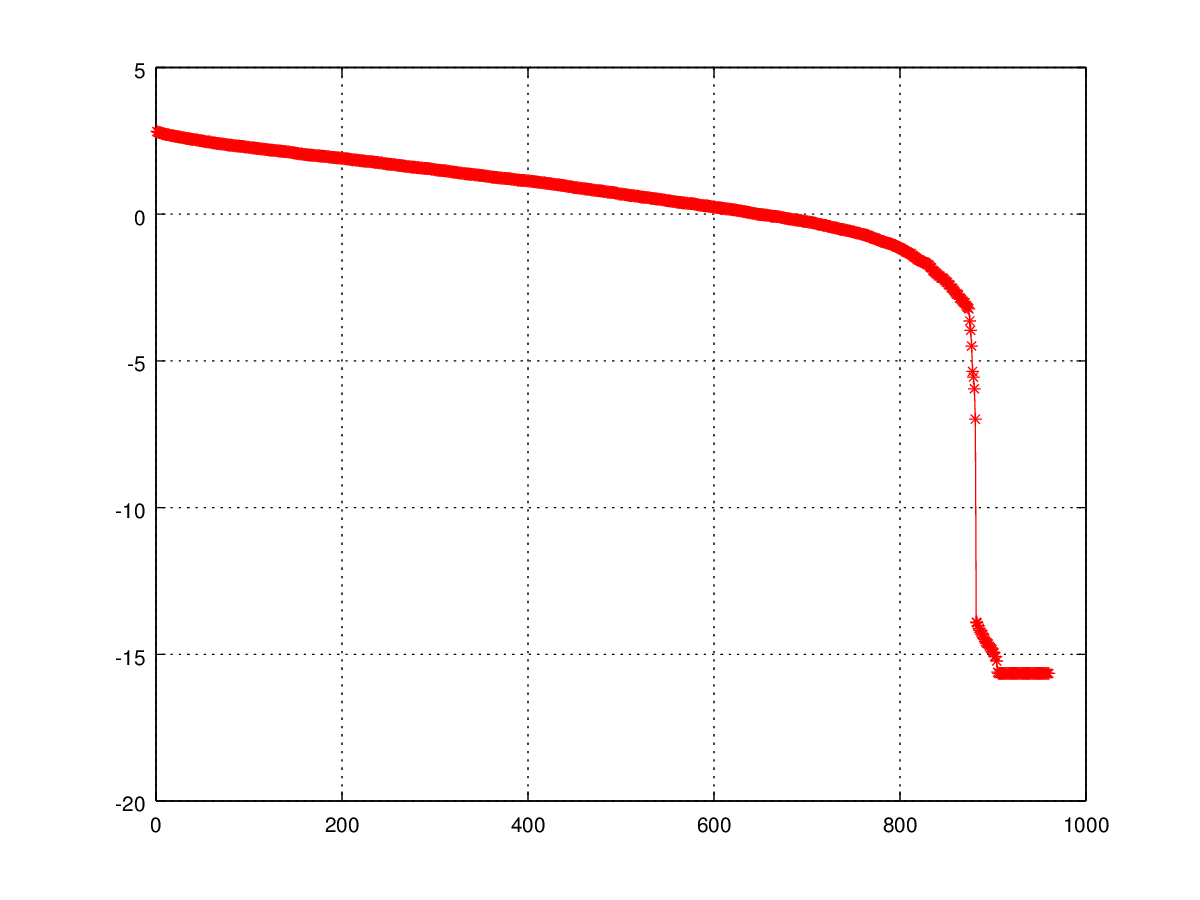
\includegraphics[width=8cm]{qrp.png}
\end{center}
 On s'aperçoit alors que les derniers éléments non nuls décroissent très vite, et qu'il peut devenir difficile de choisir un seuil au dessus duquel les éléments diagonaux seront déclarés ``non nuls''.
En d'autres termes, le ``saut'' entre éléments ``non-nuls'' et éléments proches du epsilon de la machine a tendance à diminuer à mesure que la taille de la matrice augmente, ce qui rend le calcul du rang numérique difficile.\\
Nous pouvons cependant améliorer un peu la situation précédente, en exploitant une propriété de $B(1)$. En effet, en permutant lignes et colones de cette matrice d'une certaine façon, on peut arriver à une structure bloc-triangulaire de $B(1)$.
\begin{center}
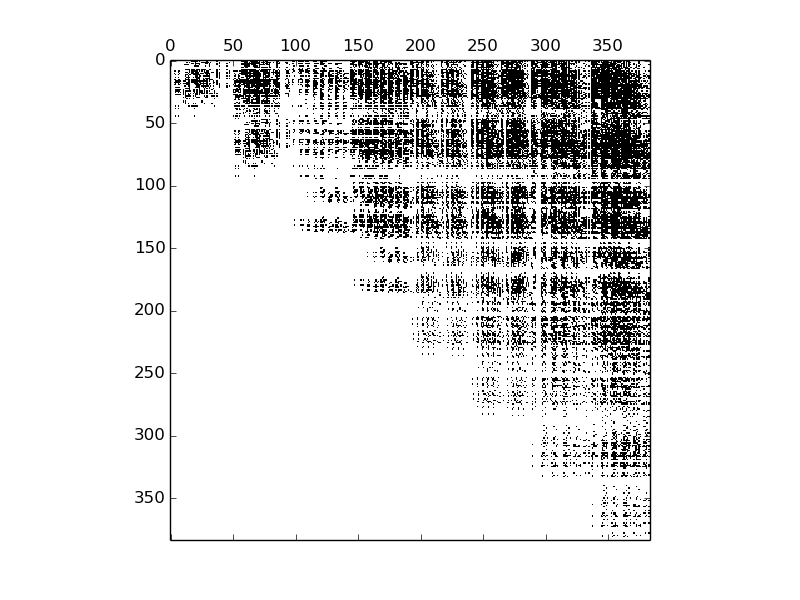
\includegraphics[width=8cm]{B0_tri.png}
\end{center}
En factorisant la matrice bloc après bloc, les éléments diagonaux vont alors décroitre uniquement à l'intérieur de chaque bloc, ce qui permet à la fin de préserver un saut numérique plus grand que dans la première approche. Le graphique ci dessous montre la nouvelle disposition des éléments diagonaux pour le même exemple que précédemment, traité de la deuxième façon.
\begin{center}
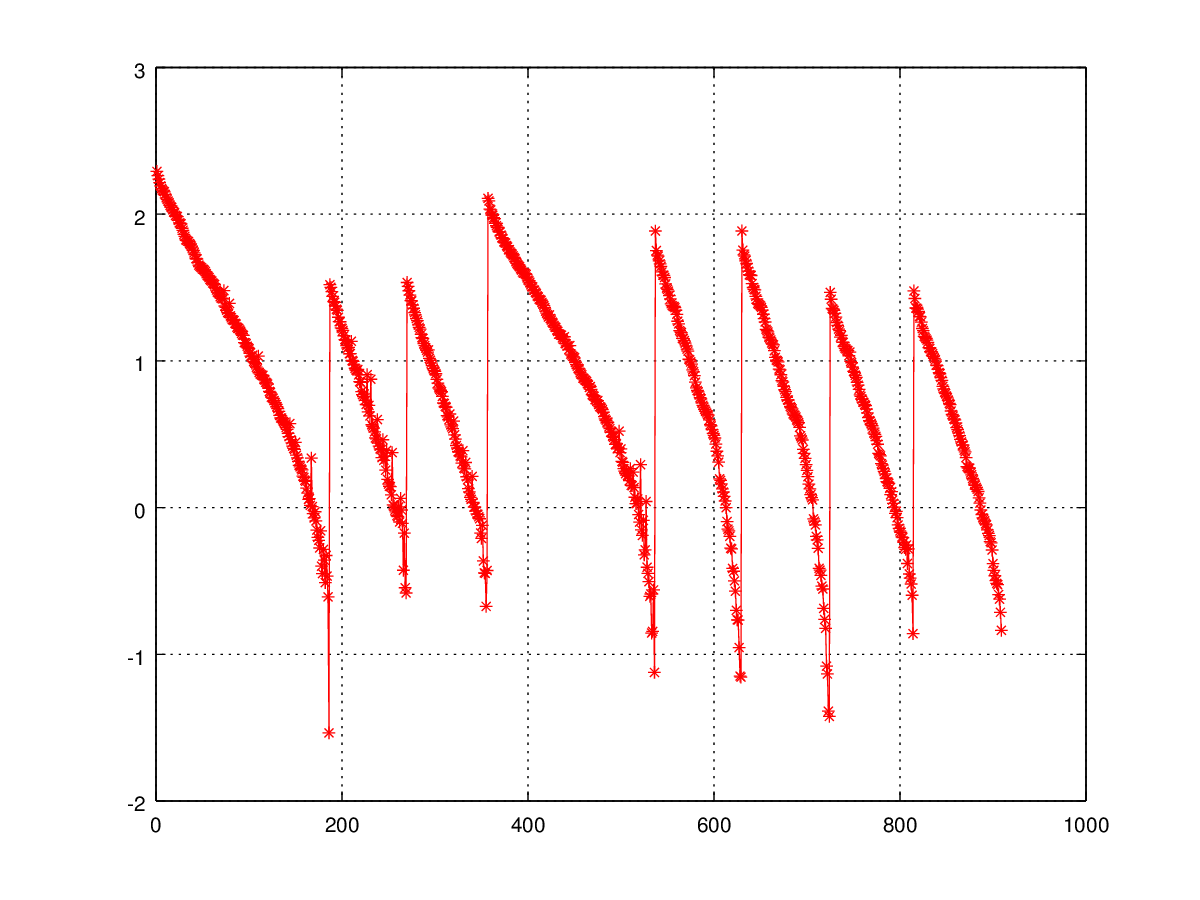
\includegraphics[width=8cm]{bloc_triang.png}
\end{center}
On voit que, malgré une décroissance rapide des éléments diagonaux dans chaque bloc, la plus petite taille de ceux-ci permet au plus petit élément ``non-nul" d'être beaucoup plus grand que le epsilon machine, ce qui facilite le calcul du rang numérique.

\end{document}
